\newpage
\section{Durchführung}

Im Folgenden werden die in \cite{krypt} beschriebenen Schritte durchgeführt und dokumentiert. Die gestellten Komponenten liegen zunächst
als Einzelteile vor und umfassen eine in \cite{Riggs_2022} beschriebene modifizierte Version des Versuchs. Neben denselben Komponenten
für rotes Licht sind darin zusätzlich zwei grüne Laser und vier weitere Sensormodule mit den zugehörigen Elektroniken enthalten. Außerdem
umfasst es zwei Strahlteilerwürfel, vier für die kürzere Wellenlänge optimierte Halbwellenplatten sowie vier dichriotische Spiegel zur
Parallelstellung der grünen und roten Laserstrahlen. Damit lassen sich nun doppelt so viele Polarisationszustände übertragen, statt
binärer können ternäre oder quartäre Zustände gewählt werden, die in einem Puls mehr Informationen enthalten. Indem Täuschzustände
definiert werden, die von den normalen Parteien nicht verwendet werden aber durch die notwendige Messung eines Lauschers unbeabsichtigt
auftreten können, lässt sich ein Abhörversuch identifizieren, ohne Schlüsselbits zu opfern.

Auf diese Ergänzung wird hier verzichtet, es kommen also nur zwei rote Laser mit ihren Elektroniken, vier Detektoreinheiten von denen
je zwei an eine Elektronik angeschlossen werden, vier Halbwellenplatten für rotes Licht, sowie zwei polarisierende Strahlteiler vor.
Diese werden nach den Anweisungen aus \cite{krypt} zur Montage auf den Steckbrettern in den entsprechenden Halterungen montiert und
stets so verbaut, dass ausreichend Platz für eine zukünftige Erweiterung um den vollständigen Aufbau gegeben ist. Von Werk aus sind
die Laser vermessen und alle Netzteile stabilisiert.



\subsection{Justierung}

Zunächst wird die ebene Ausrichtung der beiden Laser justiert. Dabei hilft eine Justierhilfe, die zur Anzeige des Strahls in geringer
und großer Entfernung genutzt werden kann. Der Laserpunkt sollte die Skala abstandsunabhängig in der gleichen Höhe treffen. Ist dies
erfolgt wird weiter die bevorzugte Polarisationsrichtung der Laser parallel zur Brettebene eingestellt. Dazu wird ein Strahlteiler mit
korrekter Orientierung in den senkrecht zu ihm verlaufenden Strahlengang gebracht und der reflektierte Teil auf einen Schirm geworfen.
Nun kann der Laser in seiner Halterung solange um die Strahlachse gedreht werden, bis die abgebildete senkrecht polarisierte Intensität 
minimal wird. In dieser Orientierung werden die Laser dann befestigt. Auf ähnliche Weise wird die Richtung der Halbwellenplatten
überprüft. Es wird je eine Polarisatorplatte zwischen Laser und Strahlteilerwürfel positioniert, die Drehskala gelöst und solange
rotiert, bis die reflektierte Intensität das Minimum erreicht. Diese Einstellung muss dann wieder fixiert werden, bevor die
Winkelanzeige ausgeschraubt und auf die Nullstelle gestellt wieder eingebaut wird. Die Polarisatoren sind also in plattenparalleler
Ausrichtung genullt, alle Komponenten sind somit einsatzbereit.



\subsection{Aufbau}

Nachdem die vorherigen Voraussetzungen erfüllt sind, kann der eigentliche Messaufbau eingerichtet werden. Das erfolgt nach dem in
Abbildung \ref{fig:schema} gezeigten Schema. Wie zuvor werden die Laser dafür zu Beginn in den Dauerbetrieb versetzt. Ohne verbaute
Strahlteiler muss der transmittierte Anteil senkrecht auf den der Null entsprechenden Sensor fallen. Anschließend wird der Strahlteiler
eingesetzt und an den Stellschrauben senkrecht zum Strahl gestellt, indem überprüft wird, ob der Laser weiterhin den Detektor trifft.
Weiter wird der Sensor, welcher der Eins entspricht, so ausgerichtet, dass der reflektierte Strahl orthogonal auf dem Detektor steht.
Um abschließend die korrekte Funktionsweise zu verifizieren, werden die Laser per Knopfdruck in den Pulsbetrieb und die Sensoren auf
Justierbetrieb geschaltet. Nun gilt es alle in Tabelle \ref{tab:kombination} eingetragenen Möglichkeiten der Polarisationsdreher auf
die richtige Leuchtkombination zu testen.

\begin{table}
	\centering
	\caption{.}
	\label{tab:kombination}
	\begin{tabular}{rccc}
		\toprule
		Sender & Empfänger & Leuchten & Bit \\
		\midrule
		\qty{-45}{\degree}\hspace{1ex} & \qty{0}{\degree} & beide & Zufall \\
		\qty{  0}{\degree}\hspace{1ex} & \qty{0}{\degree} & transmittiert & Null \\
		\qty{ 45}{\degree}\hspace{1ex} & \qty{0}{\degree} & beide & Zufall \\
		\qty{ 90}{\degree}\hspace{1ex} & \qty{0}{\degree} & reflektiert & Eins \\
		\qty{-45}{\degree}\hspace{1ex} & \qty{45}{\degree} & transmittiert & Null \\
		\qty{  0}{\degree}\hspace{1ex} & \qty{45}{\degree} & beide & Zufall \\
		\qty{ 45}{\degree}\hspace{1ex} & \qty{45}{\degree} & reflektiert & Eins \\
		\qty{ 90}{\degree}\hspace{1ex} & \qty{45}{\degree} & beide & Zufall \\
		\bottomrule
	\end{tabular}
\end{table}

Dieses Vorgehen wird zunächst ohne \glqq{Eve}\grqq{} für \glqq{Alice}\grqq{} als Sender und \glqq{Bob}\grqq{} als Empfänger ausgeführt.
Nach Aufnahme der ersten Messreihe kann \glqq{Eve}\grqq{} eingesetzt werden und wird dann sowohl für die Rolle des Senders als auch des
Empfängers kalibriert. Dabei sollte eine veränderte Einstellung von \glqq{Alice}\grqq{} und \glqq{Bob}\grqq{} vermieden werden, um die
Absicht eines zunächst unbemerkten Lauschers zu simulieren, der dann mittels der zweiten Messreihe enttarnt wird.

\begin{figure}[H]
	\centering
	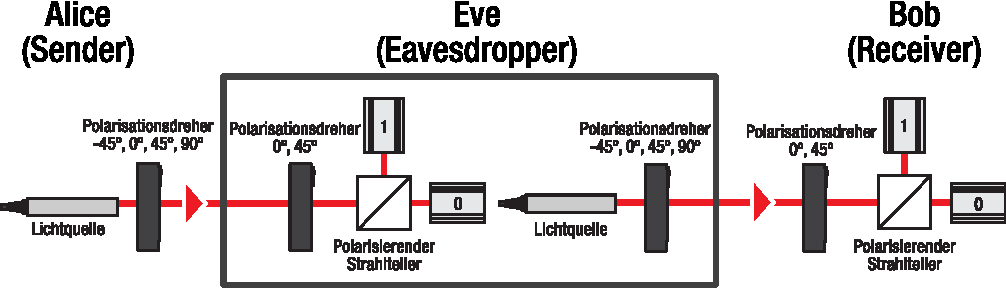
\includegraphics[width=0.9\textwidth]{content/aufbau/schema.pdf}
	\caption{. \cite{krypt}}
	\label{fig:schema}
\end{figure}

\begin{figure}[H]
	\centering
	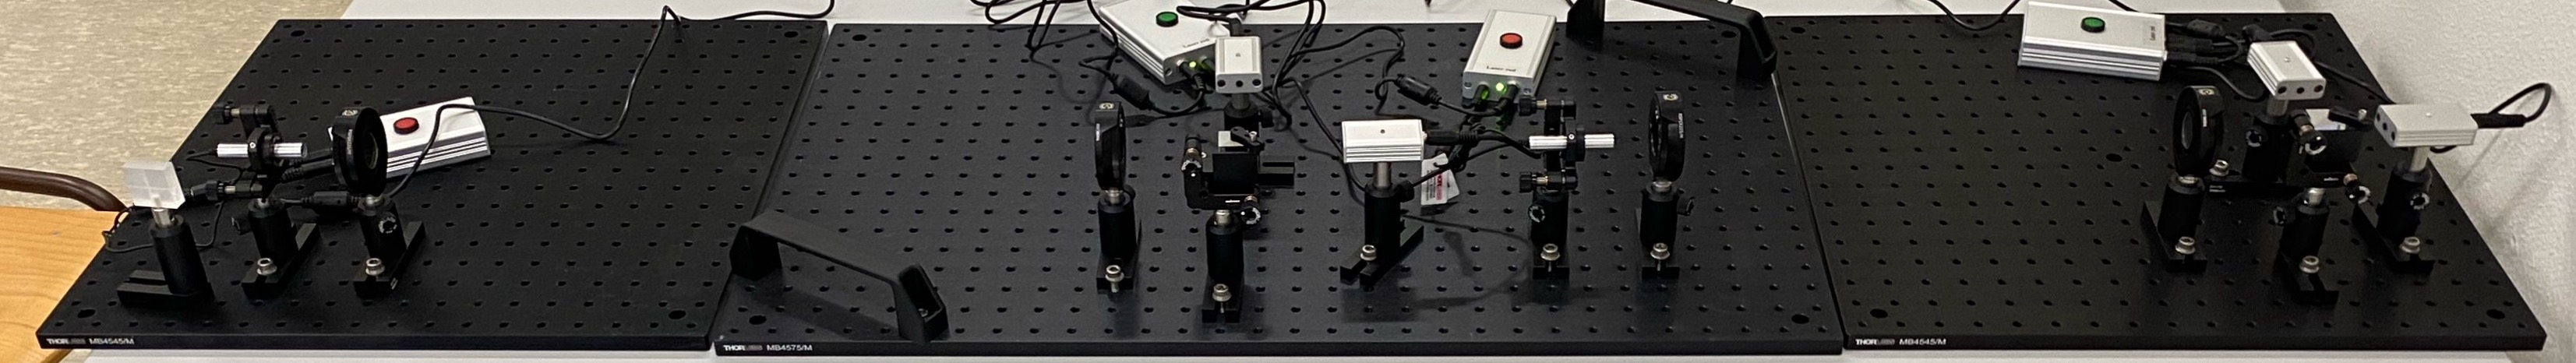
\includegraphics[width=1.0\textwidth]{content/aufbau/front.jpg}\\[1ex]
	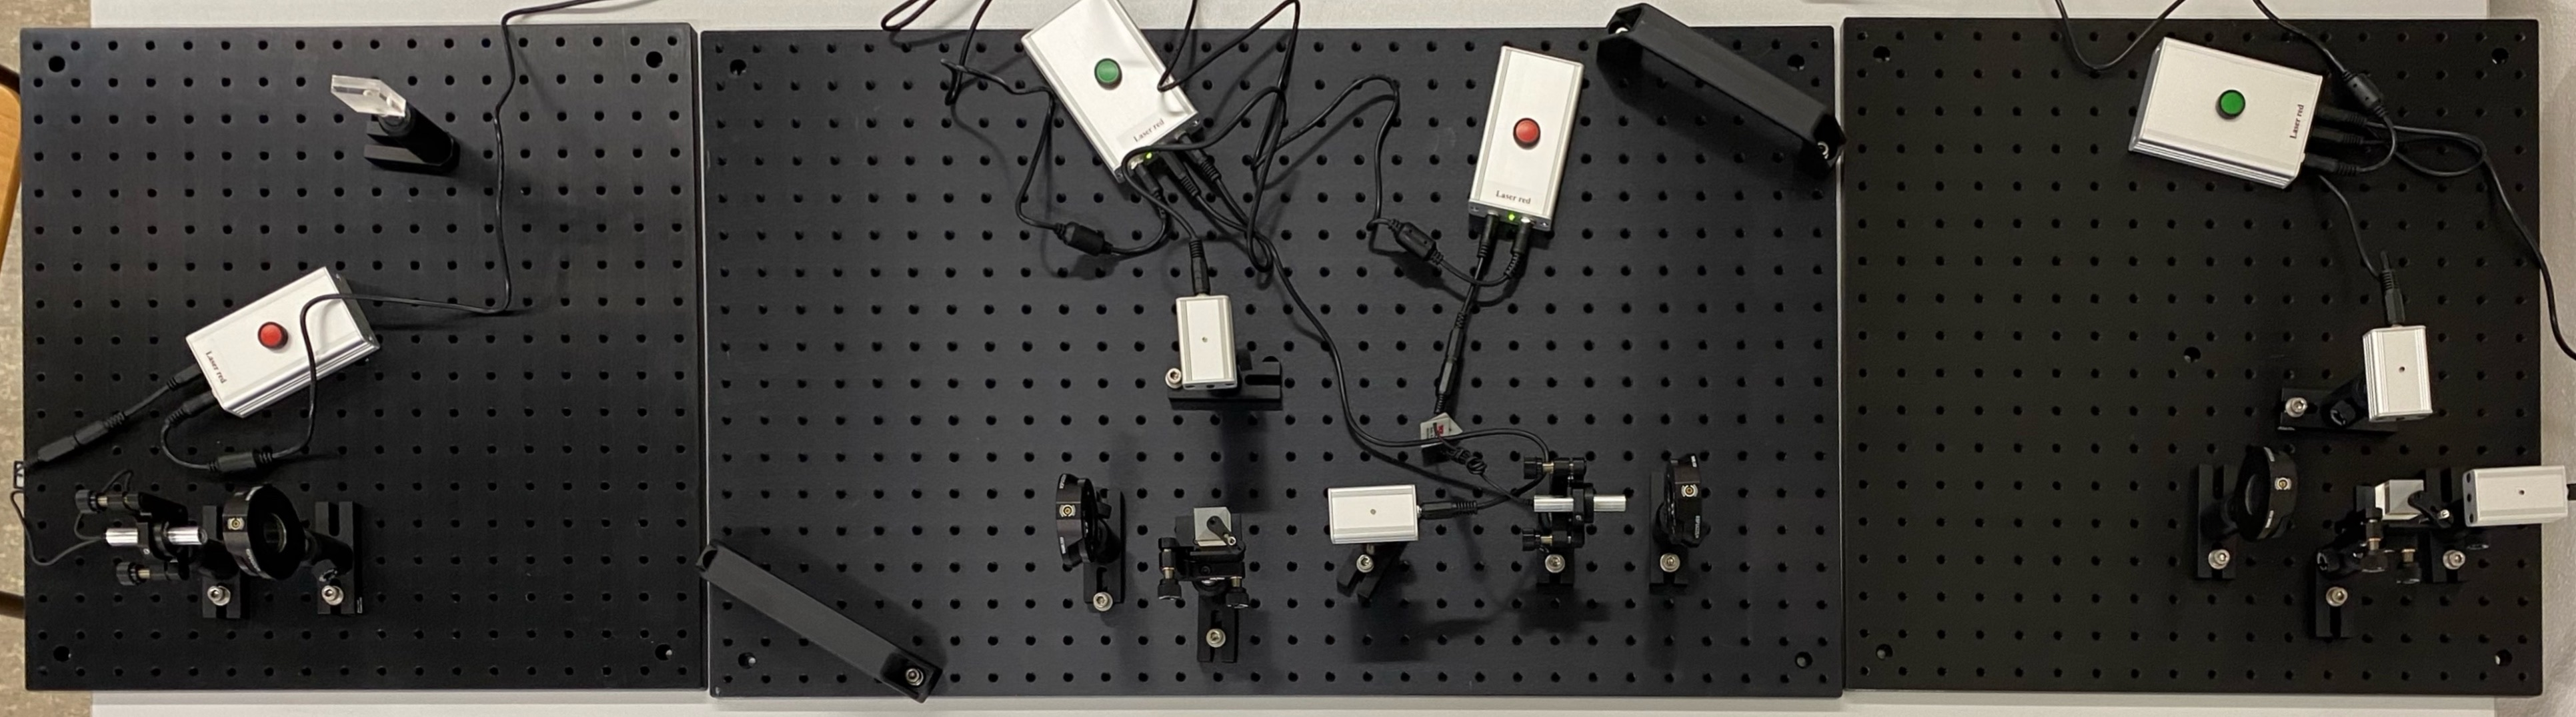
\includegraphics[width=1.0\textwidth]{content/aufbau/drauf.jpg}
	\caption{.}
	\label{fig:aufbau}
\end{figure}



\subsection{Verfahren}



\subsubsection{Verschlüsselung einer Nachricht}



\subsubsection{Identifikation eines Abhörversuchs}
